% Author: Izaak Neutelings (September 2020)
\documentclass[border=3pt,tikz]{standalone}
\usepackage{amsmath}
\usepackage{tikz}
\usepackage{physics}
\usetikzlibrary{intersections}
\usetikzlibrary{decorations.markings}
\usetikzlibrary{angles,quotes} % for pic
\usetikzlibrary{decorations.pathmorphing} % for decorate random steps
\tikzset{>=latex} % for LaTeX arrow head
\usepackage{xcolor}
\colorlet{xcol}{blue!70!black}
\colorlet{xcol'}{xcol!50!red!80!black}
\colorlet{veccol}{green!45!black}
\tikzstyle{vector}=[->,thick,veccol,line cap=round]
\tikzstyle{rvec}=[->,thick,xcol,line cap=round]

\begin{document}

% VECTOR breakdown on axis
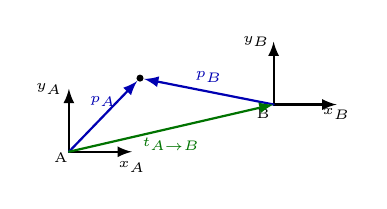
\begin{tikzpicture}
  \tikzstyle{every node}=[font=\tiny]
  \small
  \def\L{0.8}
  \def\R{1.3}
  \def\ang{46}
  \def\thet{-52}
  \coordinate (O) at (0,0);
  \coordinate (O1) at (2.6,0.6);
  \coordinate (R) at (\ang:\R);
  \node[fill=black,circle,inner sep=0.9] (R') at (R) {};
  
  % O1
  \draw[<->,thick] (\L,0) node[below] {$x_A$} --
                   (O) node[below left=-3] {A} --
                   (0,\L) node[left=-1] {$y_A$};
  \draw[rvec] (O) -- (R') node [midway, above] {$p_A$};
  
  % O1
  \begin{scope}[shift={(O1)}]
    \draw[<->,thick] (\L,0) node[below=-2] {$x_B$} --
                     (0,0) node[below left=-2] {B$$} --
                     (0,\L) node[left=-2] {$y_B$};
    \draw[rvec] (0,0) -- (R') node [midway, above] {$p_B$};
  \end{scope}
  
  \draw[rvec, green!45!black] (O) -- (O1) node [midway, below] {$t_{A\rightarrow B}$};


\end{tikzpicture}

\end{document}